\section{Yao's Protocol}

This section provides a complete description of Yao's \emph{garbled circuits protocol}, how the protocol incorporates \ac{OT}, and a discussion of the protocol's security and performance characteristics.  Though the protocol described here was first published by\cite{goldreich1987play}, the terminology used in this section follows more recent publications\cite{hazay2010efficient}. In all cases though the concepts are similar and there is a direct mapping between the two.

\begin{algorithm}[H]
    \floatname{algorithm}{Protocol}
    \caption{Yao's Garbled Circuits Protocol}
    \label{alg:yao}
    \begin{algorithmic}[1]
        \STATE \ac{P1} : generates a boolean circuit representation $c_c$ of \ac{f} that takes input $i_{P1}$ from \ac{P1} and $i_{P2}$ from \ac{P2}.
        \STATE \ac{P1} transforms $c_c$ by garbling each gate's computation table, creating garbled circuit $c_g$.
        \STATE \ac{P1} sends both $c_g$ and the values for the input wires in $c_g$ corresponding to $i_{P1}$ to \ac{P2}.
        \STATE \ac{P2} uses \emph{1-out-of-2 \ac{OT}} to receive from \ac{P1} the encrypted values for $i_{P2}$ to $c_g$.
        \STATE \ac{P2} calculates $c_g$ with the encrypted versions of $i_{P1}$ and $i_{P2}$ and outputs the result.
    \end{algorithmic}
\end{algorithm}


\subsection{Intuitive Description of the Protocol}

This section attempts to provide a high level explanation of how Yao's protocol works and some of the reasoning behind its construction. It is included to make the following detailed description of the protocol easier to follow.

\ac{P1} and \ac{P2} wish to compute function \emph{f} securely, so that their inputs to the function remain secret. They will do so by modeling \emph{f} as a boolean circuit. \ac{P1} will then ``garble'' the circuit by replacing all boolean values in the circuit with pseudo-random looking strings, and then keeping secret the mapping between these strings and the underlying boolean values. This is done for all gates in the circuit except for the output gates of the circuit.  The values of the output wires for these gates are left un-garbled.

\ac{P1} will then similarly replace each bit of his input with the pseudo-random string that maps to that bit's input into the circuit. \ac{P1} then sends the garbled circuit and the strings corresponding to his input bits to \ac{P2}.

\ac{P2} receives both the garbled circuit and \ac{P1}'s garbled input values. However, since all input wires into the circuit have been garbled and only \ac{P1} has the mapping between the garbled values and underlying bits, \ac{P2} does not know what values to input into the circuit to match her input bits.
In other words, for each input wire into the circuit, \ac{P2} can select one of two random strings to input (corresponding to 0 or 1), but does not know which of these correspond to her desired input bit.

In order to learn which pseudo-random string to select for each of \ac{P2}'s input wires, \ac{P2} engages in a \emph{1-out-of-2 \ac{OT}} with \ac{P1} for each bit of \ac{P2}'s input. For each round of the \ac{OT}, \ac{P2} submits the bit she wishes to learn, receives the corresponding string, and, \ac{P1} learns nothing.

Once \ac{P2} has received all of the strings corresponding to her input into the circuit, she holds everything needed to compute the output of the circuit, namely her garbled inputs, \ac{P1}'s garbled inputs, and the garbled circuit itself. Further, she has obtained these values without \ac{P1} learning her inputs, nor \ac{P2} learning \ac{P1}'s inputs.

\ac{P2} then begins to compute the circuit by entering the pseudo-random strings that correspond to each bit of her and \ac{P1}'s input into each corresponding input gate and using the resulting string as the input to the next gate. \ac{P2} may try to learn information about \ac{P1}'s inputs by watching the execution of the circuit. The protocol prevents \ac{P2} from doing so though the manner that each computation table for each gate was constructed.

Recall that the computation table for every gate in the circuit was constructed so that each pair of inputs produces a output string that represents the correct boolean result, but which appears pseudo-random to \ac{P2}.  In other words, instead of mapping from $\{0, 1\} x \{0, 1\} \to \{0, 1\}$, all gates in the circuit map from two random looking strings to another uniformly distributed pseudo-random string. Since \ac{P2} never learns the mapping between strings used in the table and their underlying boolean values, \ac{P2} learns nothing by watching the outputs of each gate.

Recall that the output values of the output gates in the circuit are not masked. This results in \ac{P2} learning the value of $f(i_{P1}, i_{P2})$ once the computation has finished.  \ac{P2} then shares this computed value with \ac{P1}.


\subsection{Detailed Description of the Protocol}

This section provides a more detailed explanation of how each step of Yao's protocol, specifying how each step of the protocol can be implemented.  The numbering of subsections here is intended to following the number of the protocol's steps in Protocol \ref{alg:yao}.


\subsubsection{Generating Boolean Circuit Representation of the Function}

The function \emph{f} being securely evaluated must first be converted into and equivalent boolean circuit $c$ so that $\forall x, y \in \{f(x, y) = c(x, y)\}$. The strategies for doing so are function specific, and thus is beyond the scope of the protocol.  For the purposes of this paper though, it is sufficient to note that there exists a mapping from any polynomial time function with fixed sized inputs to a boolean circuit that calculates the same output\cite{goldreich1987play}.


\subsubsection{Garbling Each Gate's Truth Table}

Once \ac{P1} has constructed the boolean circuit representation $c$ of $f$, the next step is to garble the truth table for each gate in $c$, or generating a garbled version of $c$ from the clear version of $c$ ($c_c \to c_g$).

\begin{figure}[ht!,height=2in]% [width=4in]
  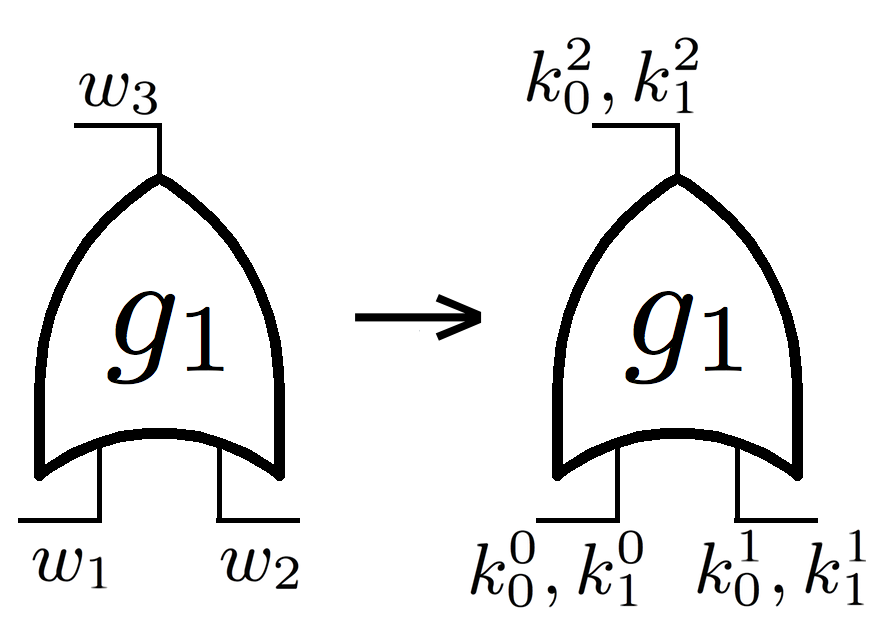
\includegraphics[width=\columnwidth]{images/and_gate}
  \caption{Garbling a single circuit}
  \label{fig:garblecircuit}
\end{figure}

To see how \ac{P1} does, this first, consider a single OR gate, $g_{OR}$
